\documentclass[../Main.tex]{subfiles}
\begin{document}
\chapter{Mechanik von Massenpunkten}

\intro{

}

\section{Gleichförmige Bewegung}

\begin{figure}[H] 
    \centering
    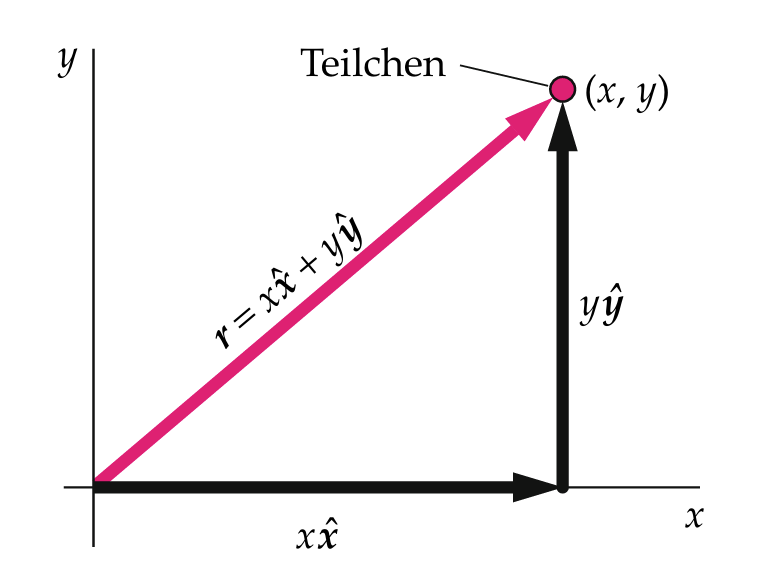
\includegraphics[width=0.5\linewidth]{Images/ortsvektor.png}
    \caption{Ortsvektor}
\end{figure}

\defn{Ortsvektor}{
    \begin{equation}
        r = x \hat{x} + y \hat{y}
    \end{equation}
}

\begin{figure}[H] 
    \centering
    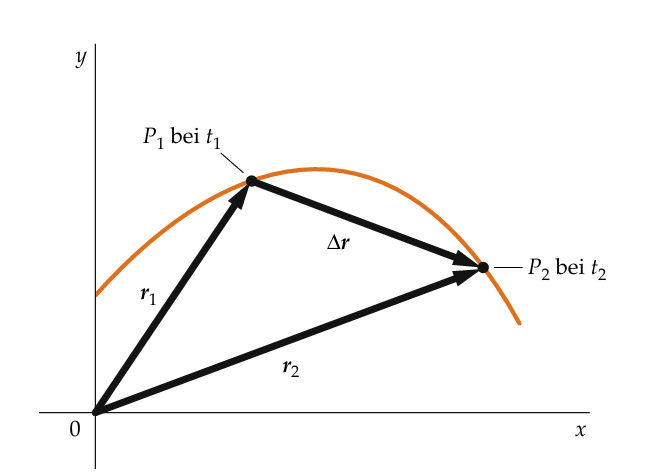
\includegraphics[width=0.5\linewidth]{Images/verschiebungsvektor.png}
    \caption{Verschiebungsvektor}
\end{figure}

\defn{Verschiebungsvektor}{
    \begin{equation}
        \Delta r = r_2 - r_1
    \end{equation}
    \begin{equation}
        \Delta r = (x_2-x_1)\hat{x}+(y_2 - y_1)\hat{y}
    \end{equation}
}

\defn{Geschwindikeit}{
    \begin{equation}
        v = \frac{\Delta r}{\Delta t}
    \end{equation}
}

\defn{Ort in Abhängigkeit der Zeit}{
    In der gleichförmigen Bewegung:
    \begin{equation}
        r(t)= v (t-t_0) + r_0 
    \end{equation}
}

\defn{Mittlerer Geschwindikeitsvektor}{
    Ist die durchschnittliche Geschwindikeit, 
    mit der sich der Körper zwischen zwei Punkten bewegt.
    \begin{equation}
        \langle v \rangle = \frac{\Delta r}{\Delta t}
    \end{equation}
}

\begin{figure}[H] 
    \centering
    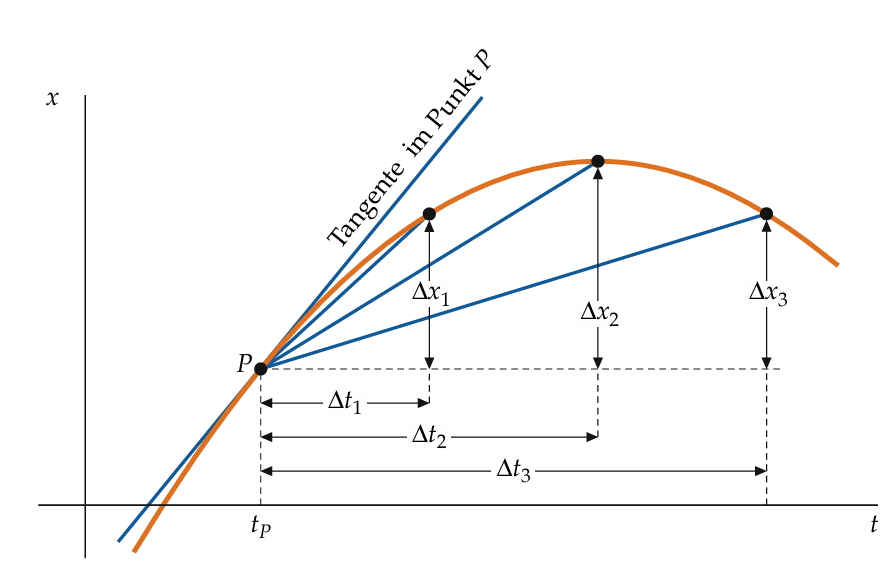
\includegraphics[width=0.75\linewidth]{Images/momentangeschwindigkeit.png}
    \caption{Momentangeschwindigkeit}
\end{figure}

\defn{Momentangeschwindigkeit}{
    \begin{equation}
        v_x(t) = \lim_{\Delta t \to 0} \frac{\Delta x}{\Delta t}
    \end{equation}
    \begin{equation}
        v(t) = \frac{dr}{dt} = \dot{r}(t)
    \end{equation}
}

\begin{figure}[H] 
    \centering
    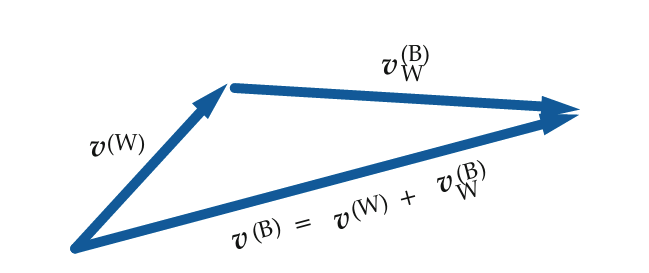
\includegraphics[width=0.75\linewidth]{Images/relativgeschwindigkeit.png}
    \caption{relativgeschwindigkeit}
\end{figure}
\defn{Relativ Geschwindigkeit}{
    Wenn sich ein Teilchen mit der Geschwindigkeit \(v^A\)
    relativ zum Bezugssystem A bewegt, das sich
    seinserseits mit der Geschwindigkeit \(v_A^B\)
    relativ zum Bezugssystem B bewegt, ist die
    Geschwindigkeit des Teilchens relativ zum Bezugssystem B:
    \begin{equation}
        v^B = v^A + v_A^B
    \end{equation}
}

\defn{Momentanbeschleunigung}{
    \begin{equation}
        a(t) = \lim_{\Delta t \to 0} \frac{\Delta v}{\Delta t}
    \end{equation}
}

\defn{Beschleunigung}{
    \begin{equation}
        \langle a \rangle = \frac{\Delta v}{\Delta t}
    \end{equation}
}

\begin{figure}[H] 
    \centering
    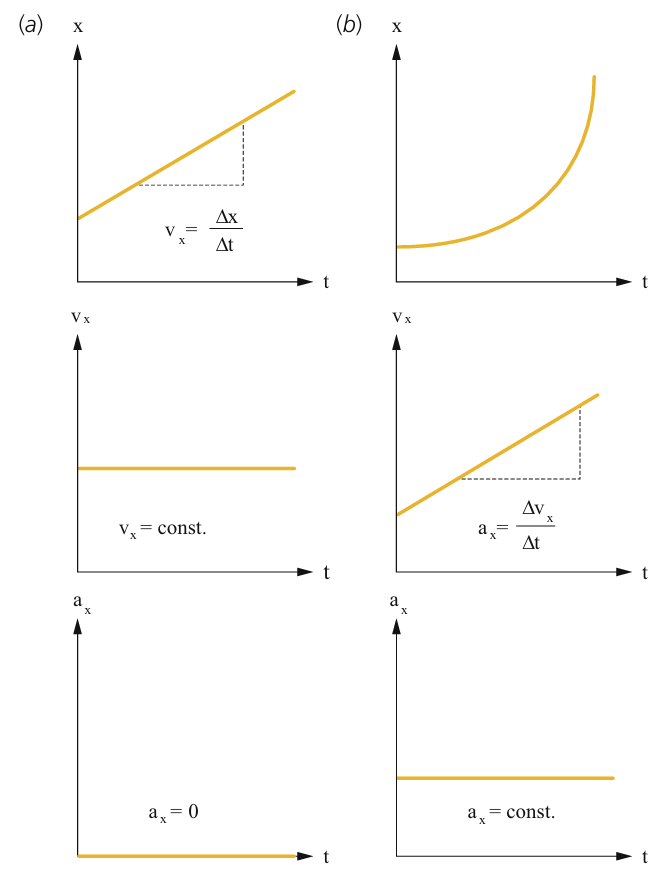
\includegraphics[width=0.75\linewidth]{Images/weg-zeit-gleichbeschleunigte-bewegung.png}
    \caption{Weg-Zeit Diagramm der gleichbeschleunigten Bewegung}
\end{figure}

\section{Kinematische Gleichungen für gleichförmig beschleunigte Bewegung}
\defn{Geschwindigkeit}{
    \begin{equation}
        v = v_0 + at
    \end{equation}
}
\defn{Mittlere Geschwindigkeit}{
    \begin{equation}
        \langle v \rangle = \frac{1}{2}(v_0+v)
    \end{equation}
}

\defn{Verschiebung durch a}{
    \begin{equation}
        \Delta x = x-x_0 = v_0 t + \frac{1}{2} a t^2
    \end{equation}
}

\defn{Verschiebung durch \(\langle v \rangle\)}{
    \begin{equation}
        \Delta x = x - x_0 = \langle v_x \rangle t = \frac{1}{2} (v_0 + v)t
    \end{equation}
}

\defn{Geschwindigkeit ausgedrückt in Beschleunidung und Delta}{
    Bei konstanter Beschleunigung:
    \begin{equation}
        v^2 = v_0^2 + 2 a \Delta r
    \end{equation}
}

\defn{Ortsfunktion der gleichförmig beschleunigten Bewegung}{
    \begin{equation}
        x-x_0 = v_0 t + \frac{1}{2} a t^2
    \end{equation}
}

\section{Schräger Wurf ohne Widerstand}
\defn{Schräger Wurf}{
    \begin{equation}
        \begin{split}
            x(t) &= x_0 + v_0 t\\
            y(t) &= y_0 + v_0 t - \frac{1}{2} g t^2
        \end{split}
    \end{equation}
    Parabelgleichung:
    \begin{equation}
        y(x) = (\tan \theta_0)x - (\frac{t}{2 v_0^2 cos^2 \theta_0}) x^2
    \end{equation}
    Horizontale Reichweite:
    \begin{equation}
        R = \frac{v_0^2}{g} \sin 2\theta_0
    \end{equation}
    Vektorgleichung:
    \begin{equation}
        r = r_0 + v_0 t - \frac{1}{2}g t^2 \hat{y}
    \end{equation}
}

\section{Krummlinige Bewegung}
\defn{Zentripetalbeschleunigung}{
    \begin{equation}
        a_{ZP} = -\frac{v^2}{r}\hat{r}
    \end{equation}
}

\defn{Periode}{
    \begin{equation}
        v = \frac{2\pi r}{T}
    \end{equation}
}

\begin{figure}[H] 
    \centering
    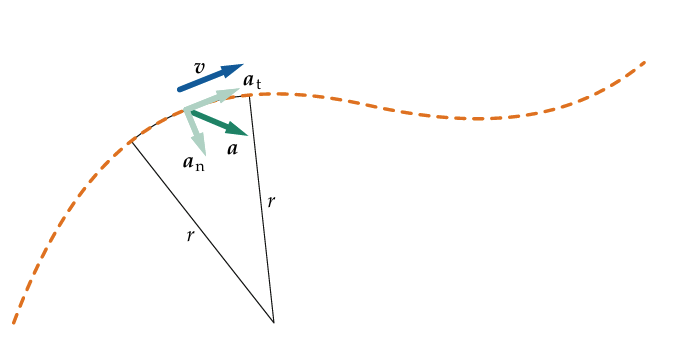
\includegraphics[width=0.75\linewidth]{Images/normal-tangential-beschleunigung.png}
    \caption{Normal- und Tangentialbeschleunigung}
\end{figure}
\defn{Normal- und Tangentialbeschleunigung}{
    \begin{equation}
        \begin{split}
            a_n &= \frac{v^2}{r} \hat{n} \\
            a_t &= \frac{dv}{dt} \hat{t}
        \end{split}
    \end{equation}
}

\end{document}
